\documentclass[a4paper]{ltjsarticle}
\usepackage[a4paper]{listings,jvlisting}
\usepackage{graphicx}

\lstset{
  basicstyle={\ttfamily},
  identifierstyle={\small},
  commentstyle={\smallitshape},
  keywordstyle={\small\bfseries},
  ndkeywordstyle={\small},
  stringstyle={\small\ttfamily},
  frame={tb},
  breaklines=true,
  columns=[l]{fullflexible},
  numbers=left,
  xrightmargin=0,
  xleftmargin=3,
  numberstyle={\scriptsize},
  stepnumber=1,
  numbersep=1,
  lineskip=-0.5ex
}

\renewcommand{\lstlistingname}{list}
\begin{document}

\title{プログラミング技法2\_課題11}
\author{阪田征之助}
\maketitle
\newpage
\section*{課題11-1}
\subsection*{ソースコード}
課題11-1のソースコードの主要部をlist\ref{kadai1}に示す。

\begin{lstlisting}[caption=kadai11-1.py,label=kadai1]
    def class_average(X, y, img_size):
    A = []
    for i in range(10):
        x = X[y == i]
        x = x.mean(0)
        A.append(x.reshape(img_size))
    return A
\end{lstlisting}
Xがnumpy.arrayであるためリストで値を返しても良いと判断し,自分が思う簡潔なコードとなった。
\\結果は最終ページに記す。

\newpage

\section*{課題11-2}
\subsection*{ソースコード}
課題11-2のソースコードの主要部をlist\ref{kadai2}に示す。
\begin{lstlisting}[caption=kadai11-2.py,label=kadai2]
    def cross_validate(clf_type, X, y, cv):

        if clf_type == 'kNN':
            clf = sklearn.neighbors.KNeighborsClassifier()
        if clf_type == 'MLP':
            clf = sklearn.neural_network.MLPClassifier()
        if clf_type == 'NaiveBayes':
            clf = sklearn.naive_bayes.GaussianNB()
        if clf_type == 'SVM':
            clf = sklearn.svm.SVC()
        scores = sklearn.model_selection.cross_validate(clf, X, y, cv=cv, return_train_score=True)
    
        return scores['train_score'],scores['test_score']
\end{lstlisting}
サンプルコードからコードを書いたため引数が何であるかを理解するのに時間がかかった。とても冗長なコードになったが動けばよしの気持ちで行きます。

\subsection*{出力結果}
課題11-2の出力結果をlist\ref{result2}に示す。
\begin{lstlisting}[caption=output, label=result2]
    Performed by kNN
        Train score:    99.05%
        Test score:     97.11%
    Performed by MLP
        Train score:    100.00%
        Test score:     95.55%
    Performed by NaiveBayes
        Train score:    86.18%
        Test score:     81.14%
    Performed by SVM
        Train score:    99.67%
        Test score:     97.00%
\end{lstlisting}
結果より正しく動いていることがわかる。kNNでも高い精度が出るのだと感心した。
\newpage

\section*{課題11-3}
フォントは数字70128882\( https://pixta.jp/illustration/70128882 \)を使用している。
\subsection*{ソースコード}
課題11-3のソースコードの主要部をlist\ref{kadai3}に示す。
\begin{lstlisting}[caption=kadai11-3.py, label=kadai3]
    def load_img(test_img_number):
        img = Image.open(str(test_img_number)+'.jpg')
        img_gray = img.convert('L')
        img_invert = ImageOps.invert(img_gray)
        img_resize = img_invert.resize(img_size)
        img_array = np.array(img_resize)/16
        img_reshape = img_array.reshape([-1, np.prod(img_size)])
        return np.array(img_reshape[0])
\end{lstlisting}
データの名前を'num'+.jpgにすることによって引数から画像を読み込んでいる。

\subsection*{出力結果}
課題11-3の出力結果をlist\ref{result3}に示す。
\begin{lstlisting}[caption=output, label=result3]
    Test class 0 image --> classified into class 4.
    Test class 1 image --> classified into class 1.
    Test class 2 image --> classified into class 8.
    Test class 3 image --> classified into class 3.
    Test class 4 image --> classified into class 4.
    Test class 5 image --> classified into class 4.
    Test class 6 image --> classified into class 4.
    Test class 7 image --> classified into class 7.
    Test class 8 image --> classified into class 8.
    Test class 9 image --> classified into class 9.
\end{lstlisting}
1,3,4,7,8,9が正しく識別できた。プログラムは正しく動いたことがわかったが精度としてはイマイチな結果となった。

\newpage
最後に本課題で使用したデータを以下に示す。
\begin{center}
    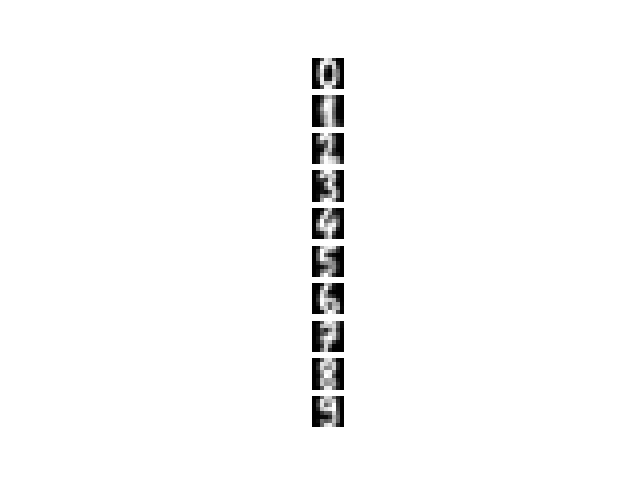
\includegraphics{output11-1.png} \\
    図1 課題11-1結果\\
    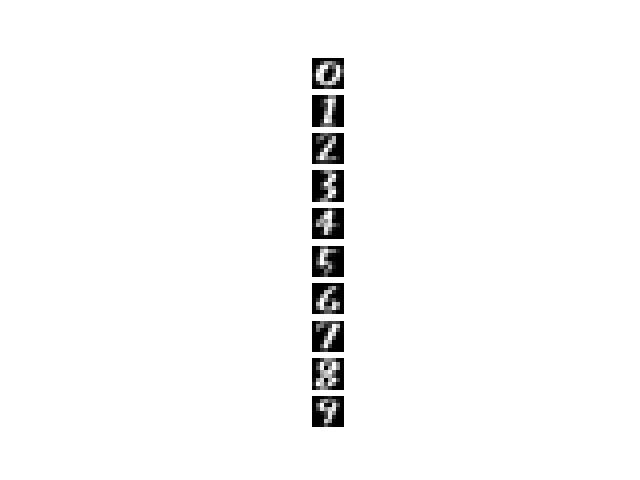
\includegraphics{output11-3.png} \\
    図1 課題11-3結果
\end{center}
\end{document}